\documentclass{bioinfo}
\copyrightyear{2015}
\pubyear{2015}

\begin{document}
\firstpage{1}

\title[VALET]{VALET: \emph{de novo} pipeline for finding metagenomic mis-assemblies}
\author[Hill \textit{et~al}]{Christopher Michael Hill\,$^{1,2,*}$, Jonathan Gluck\,$^{1}$, Victoria Cepeda\,$^{1,2}$, Matheiu Almedia\,$^{2}$, Sergey Koren\,$^{1,2}$, Atif Memon\,$^{1}$, and Mihai Pop\,$^{1,2}$\footnote{to whom correspondence should be addressed}}
\address{$^{1}$Department of Computer Science,
University of Maryland, College Park, Maryland, 20742
USA\\ $^{2}$ Center
for Bioinformatics and Computational Biology, University of
Maryland, College Park, Maryland, 20742 USA.}

\history{Received on XXXXX; revised on XXXXX; accepted on XXXXX}

\editor{Associate Editor: XXXXXXX}

\maketitle

\begin{abstract}

\section{Motivation:}
Text Text Text  Text Text Text Text Text Text Text Text
Text  Text Text Text Text Text Text Text Text Text  Text Text Text Text Text Text Text Text Text  Text Text Text Text Text Text Text Text Text  Text Text Text Text Text Text Text Text Text  Text Text Text Text Text Text Text Text Text  Text Text Text Text Text.

\section{Results:}
Text  Text Text Text Text Text Text Text Text Text  Text Text Text Text Text Text Text Text Text  Text Text Text Text Text Text Text Text Text  Text Text Text Text Text Text

\section{Availability:}
Text  Text Text Text Text Text Text Text Text Text  Text Text Text Text Text Text Text Text Text  Text Text Text Text Text Text Text Text Text  Text

\section{Contact:} \href{name@bio.com}{name@bio.com}
\end{abstract}

\section{Introduction}
%Metagenomics is characterizing the environment around us.

Genome assembly of single organisms is made difficult due to the presence of sequencing errors and repeats.
This difficulty is compounded in metagenomic samples due to the addition of varying organism abundances, intrapopulational variations, and conserved genomic regions between closely-related species.
Since many downstream applications rely on these assembled genomes, it is critical that the assembly is error-free.
Existing methods for finding mis-assemblies have primarily focused on single genome assembly and fall into two categories: reference-based and \emph{de novo} evaluation.

Reference-based methods rely on having a collection of, often manually curated, reference genomes, while \emph{de novo} methods look for inconsistencies between characteristics of the data generation process and the resulting assembly.
QUAST~\citep{gurevich2013quast} is a tool that can identify mis-assemblies and structural variants when provided with a reference genome.
QUAST leverages existing methods (Plantagora~\citep{barthelson2011plantagora},
GeneMark.hmm~\citep{lukashin1998genemark}, GlimmerHMM~\citep{majoros2004tigrscan}) and quality metrics (GAGE~\citep{salzberg2011gage}).
QUAST uses the Plantagora’s definition of a mis-assembly,
i.e., a mis-assembly breakpoint is defined as a position in the assembled contigs where (1) the left flanking
sequence aligns over 1kb away from right flanking sequence on the reference, or (2) the sequences overlap by
over 1kb, or (3) the right flanking sequence aligns on opposite strands or different chromosomes.

\emph{De novo} techniques for detecting mis-assemblies in single genomes rely on looking for inconsistencies between the sequence generation process and the resulting assembly.
In other words, given a model of the sequencing process, could the sequences have been generated if the assembly was the truth (inserted into the sequencing machine)?
Regions of the assembly that do not meet these assumptions are signatures of potential mis-assemblies.
One assumption is that the sequence generation process is roughly uniform, i.e., sequences starting at any position have equal probability.
Substantially divergent coverage may indicate mis-assembly.
If the sequences are paired-end or mate-pair then additional constraints based on insert size can be used.

Amosvalidate~\citep{amosvalidate2008} is a \emph{de novo} pipeline for detecting mis-assemblies that incorporates the above constraints.
As mentioned in the previous chapter, REAPR~\citep{hunt2013reapr} is a tool that leverages insert size constraints and evaluates the accuracy of the assembly using read-pair coverage.
REAPR determines the fragment coverage by first independently aligning the read-pairs to the assembly.
A fragment is defined as the distance from the end points of proper read-pairs (those that are determined to have correct orientation and separated by the correct distance).
REAPR is able to find base-level errors by comparing the fragment coverage of a given base with the theoretical coverage.

Although all the above-mentioned tools were designed to work on single genomes, they do not function correctly on metagenomic assemblies.
QUAST relies on the existence of reference genomes, which are simply not available for most metagenomic samples.
Furthermore, if the \emph{correct} reference strain is not available, then QUAST may erroneously flag correct and biologically novel sequence as mis-assembled.
The \emph{de novo} tools REAPR and amosvalidate rely on global uniform sequence coverage to flag regions.
In previous chapters, we have shown that contigs within the metagenomic assemblers vary widely in abundances.
Assuming uniform coverage will cause these tools to erroneously flag regions as mis-assembled.
In this chapter, we detail how to modify the constraints of existing tools to allow them to work with metagenomic assemblies.
The result is VALET, the first \emph{de novo} pipeline for detecting mis-assemblies in metagenomic assemblies.

\section{Methods}

\subsection{Types of mis-assemblies}

The majority of mis-assemblies fall into two categories: (1) compression/expansion of repetitive sequence and (2) sequence rearrangements.
The first category of mis-assembly results when an assembler is unable to determine the correct copy count of repeats, leading to additional or fewer copies.
The second category results when an assembler erroneously links separate unique portions of the genome that lie adjacent to a repeat.
The repeat acts as a bridge joining the two separate parts of the genome together.
Each category of mis-assembly has its own signatures that can be used to identify potential mis-assemblies.

The sequencing process of randomly-sheared fragments follows a Poisson distribution~\citep{lander1988genomic}.
Regions within the assembly that show high variance in \textbf{depth of coverage} are a potential signature of compressed/expanded repeats, chimeric contigs, and other types of contamination.

The reads given to the assembler should be \textbf{alignable} to the resulting assembly.
%During sequencing, reads are produced starting from random locations within the genome.
%Thus, the reads must be able to align to the resulting assembly.
In practice, however, a read may fail to align for a few reasons.
%When a read is unable to align to an assembly, there must be some explanation.
In metagenomic samples, an unaligned read can be from a rare, low coverage organism, and was never assembled with any other reads.
A read with a large amount of errors will be unable to align within a specified similarity to the assembly.
A read can be sequenced from a unfiltered contaminant or primer.
If a read does not fall into one of the above categories, then it may be a sign of a potential mis-assembly.

Another signature that is used to find mis-assemblies relies on finding regions of the assembly that violate mate-pair \textbf{insert size constraints}.
Certain sequencing technology allows researchers to sequence from the ends of a DNA fragment of a known insert size.
Although the sequence technology can only give the raw sequence of the first couple hundred basepairs from the ends of the fragment, the distance between the ends of the sequences can be used to aid in resolving repeats, and orienting and scaffolding contigs.
Regions of an assembly containing a disproportionate number of mate-pairs (reads from the same fragment) with incorrect insert sizes may be a potential mis-assembly.

VALET flags regions of the assembly based on (1) sampling depth, (2) alignability of the sequences, and (3) insert size constraints.

\subsection{Estimating contig abundances using $k$-mers}

An important part of most metagenomic pipelines is determining the relative abundance of each contig.
The presence of repeats among different species poses a serious problem for estimating abundances.
Short-read alignment tools such as Bowtie2 often randomly assign sequences that align equally well to multiple positions ignoring the relative abundances of the underlying contigs.
This poses a \emph{chicken or the egg} type problem because the sequence alignments are used to determine the contig abundances.
Here we solve this problem by using the uniquely alignable sequences to establish an initial contig abundance.
Then when we encounter a sequence that can align multiple locations, we randomly assign it based on the relative abundance of the corresponding contigs.
We update the contig abundances and repeat the above step for a given number of iterations (30 by default).
This approach is similar in spirit to that of Sailfish~\citep{patro2014sailfish} which performs alignment-free abundance estimation of RNA-seq reads.

\subsection{Depth of coverage analysis}
%The sequencing process of randomly-sheared fragments follows a Poisson distribution~\citep{lander1988genomic}.  Regions within assembled contigs that show high variance in coverage may be potential mis-assemblies.  Areas of high and low depths of coverage could be compressed/expanded repeats, chimeric contigs, and other types of contamination.

In order to find regions of unexpectedly high/low coverage, we first learn the distribution of per-base coverages across a given contig.  Using this distribution, bases are marked if their coverage falls below or above a certain threshold.  We set the lower cutoff as the first quartile minus 1.5 $\times$ the interquartile range (IQR), which is the difference between the first and third quartile. 1.5 $\times$ IQR is the value used by Tukey’s box plot~\citep{mcgill1978variations}.  Regions whose coverage is greater than the third quartile plus 1.5 $\times$ IQR are marked as high coverage.
%The main benefit of this approach is that it is completely data-dependent. No prior assumptions of the distribution of the quality values need to be made.

Using the per-base coverages may result in a large number of regions erroneously marked as mis-assemblies due to the inherent noisiness of the data, so we also provide a sliding window approach to smooth out the per-base coverages. The larger the window, the fewer the regions marked as mis-assemblies.
VALET uses a window size of 300 bp by default.

\subsection{Insert size consistency}

%Certain sequencing technology allows researchers to sequence from the ends of a DNA fragment of a known insert size.  Although the sequence technology can only give the raw sequence of the first couple hundred basepairs from the ends of the fragment, the distance between the ends of the sequences can be used to aid in resolving repeats, and orienting and scaffolding contigs.  Regions of an assembly containing a disproportionate number of mate-pairs (reads from the same fragment) with incorrect insert sizes may be a potential mis-assembly.

VALET relies on the REAPR~\citep{hunt2013reapr} pipeline to identify mate-pair insert size inconsistencies.  REAPR works by first sampling the fragment coverage across the genome to get average fragment length and depth of coverage.  Using this information, REAPR scans the assembly for observed regions that differ from the expected fragment length distribution and orientations.

REAPR is designed to work with single genome assemblies, more specifically, assemblies with a global uniform coverage.  Since the contig abundances can vary drastically in metagenomic assemblies, VALET first bins contigs by similar abundances and then executes the REAPR pipeline on the binned contigs.

\subsection{Identifying assembly breakpoints}
% The reads given to the assembler should be alignable to the resulting assembly.
% %During sequencing, reads are produced starting from random locations within the genome.
% %Thus, the reads must be able to align to the resulting assembly.
% In practice, however, a read may fail to align for a few reasons.
% %When a read is unable to align to an assembly, there must be some explanation.
% In metagenomic samples, an unaligned read can be from a rare, low coverage organism, and was never assembled with any other reads.
% A read with a large amount of errors will be unable to align within a specified similarity to the assembly.
% A read can come from a unfiltered contaminant or primer.
% If a read does not fall into one of the above categories, then it may be a sign of a potential mis-assembly.

Possible breakpoints in the assembly are found by examining regions where a large number of partial reads are able to align.
We evenly split each unaligned read into \emph{sister} reads.
The \emph{sister} reads are then aligned independently back to the reference genome.
We partition the provided assembly into bins (100 bp by default) and record which bins correspond to the sister reads.
If we find a pair of bins that contain at least two different pairs of \textit{sister} reads, then we mark it as a breakpoint location.

\subsection{Comparing multiple assemblies}

We visualize the quality of an assembly by recording the number of errors accumulated as we add contigs in decreasing order of length.
This allows us to visually compare a set of metagenomic assemblies.

\subsection{VALET pipeline}

VALET takes as input a metagenomic assembly \textsc{FASTA} file and a collection of paired and un-paired reads (Figure~\ref{fig:valet_pipeline}).
Assembled contigs are first filtered out based on size (2x the average read length by default).
Next the abundances of contigs are calculated using our k-mer-based approach described above.
Contigs undergo an additional filtering step based on abundance (10x by default).
Higher coverage and longer sequence provide a better baseline for detecting mis-assemblies.

Once filtering has finished, regions of the assembly are flagged based on the inconsistencies described above.
In practice, most mis-assembly signatures have high false positive rates which can be reduced by looking at regions where multiple signatures agree.
%Regions that share multiple mis-assembly signatures may be more likely an \textit{actual} mis-assembly.
Therefore, any window of the assembly (2000 in length by default) that contains multiple mis-assembly signatures are marked as \textbf{suspicious}.
The flagged and suspicious regions are stored in a \textsc{GFF} file, which allows users to visualize the mis-assemblies using any genomic viewers, such as \text{IGV}~\citep{thorvaldsdottir2012integrative}.

\begin{figure*}[tb!]
\begin{center}
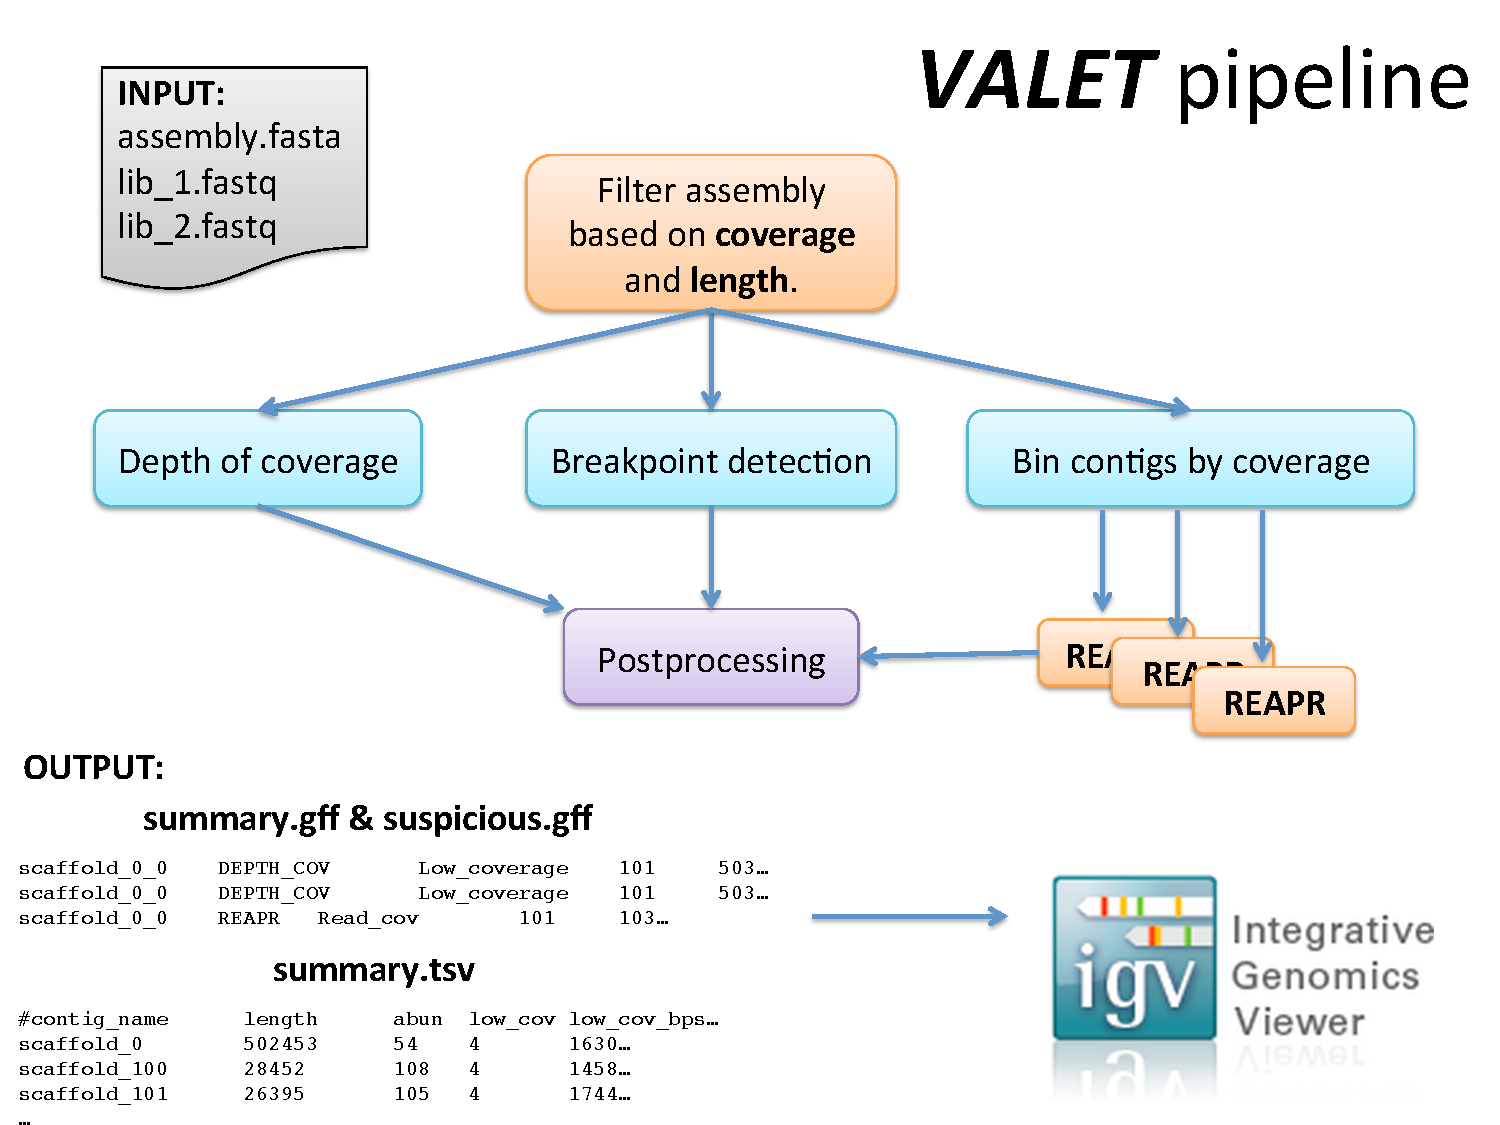
\includegraphics[width=4.86in]{figures/valet_pipeline}
\end{center}
\caption[Overview of the VALET pipeline]{Overview of the VALET pipeline.}
\label{fig:valet_pipeline}
\end{figure*}

\section{Results}

\subsection{VALET achieves high sensitivity on a simulated metagenomic community}
%Evaluating correctness – mock even/staggered/mixture of known communities.
%Examining error composition of all HMP data sets.
%Grab a handful to compare with new assemblies.
%Show that window length doesn’t matter when comparing.
%Does window length matter when comparing assemblies.

We examine the sensitivity of VALET on a toy simulated metagenomic community consisting of four bacteria at varying abundances: \emph{Bacteroides vulgatus} (80x), \emph{Bacillus cereus} (60x), \emph{Actinomyces odontolyticus} (40x), and \emph{Acinetobacter baumannii} (20x).
Approximately four million reads are simulated using \textsc{wgsim}~\citep{li2013wgsim} with default parameters.
The dataset was assembled using IDBA-UD~\citep{peng2012idba}, MetaVelvet~\citep{namiki2012metavelvet}, SPAdes~\citep{bankevich2012spades}, and SOAPdenovo2~\citep{luo2012soapdenovo2}.
We ran VALET on the assemblies and compared the errors found with the reference-based mis-assemblies detected by QUAST (Table~\ref{simulated_community} and Figure~\ref{fig:mock_frc}).
If any part of a region flagged by VALET overlaps with a mis-assembled region reported by QUAST, we consider it a true positive (mis-assembly correctly identified by our method).
%In addition, the N50 of each assembly is recalculated after breaking at mis-assemblies found by QUAST.

Across all assemblers, VALET detects greater than 80\% of mis-assemblies detected by QUAST.% with all mis-assemblies being found in the IDBA-UD and SOAPdenovo2 assemblies.
%IDBA-UD, MetaVelvet, and SPAdes assemblies contain roughly the same amount of sequence (16.3-16.5 Mbp), while SOAPdenovo2 contains roughly 4 Mbp less.
IDBA-UD has the greatest N50 after breaking the assembly at regions marked by QUAST (206.7 Kbp), followed by SPAdes (128.1 Kbp), MetaVelvet (29.5 Kbp), and SOAPdenovo2 (10.8 Kbp).
%IDBA-UD has the greatest NA50 (208.8 Kbp), followed by SPAdes (130.9 Kbp), MetaVelvet (29.5 Kbp), and SOAPdenovo2 (10.8 Kbp)
These rankings match those provided by VALET (Figure~\ref{fig:mock_frc}).



\begin{figure}[tb!]
\begin{center}
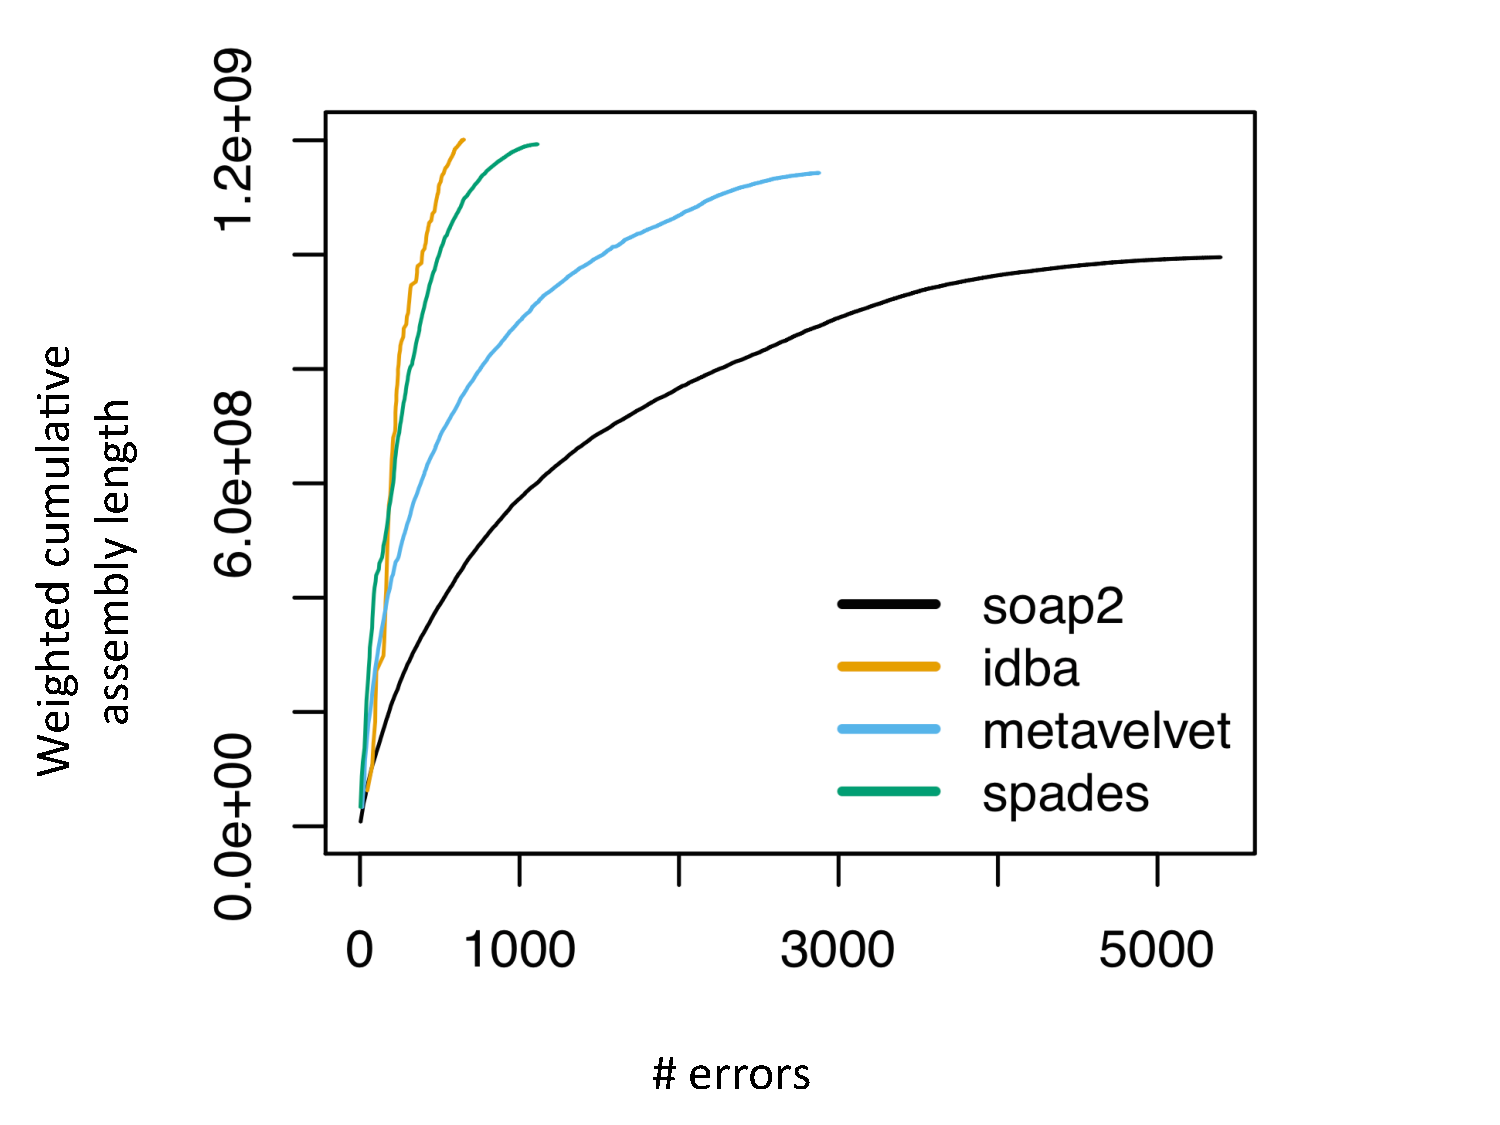
\includegraphics[width=3.86in]{figures/mock_frc}
\end{center}
\caption[RC plot of a simulated mock community]{FRC plot provided by VALET of a simulated mock community.}
\label{fig:mock_frc}
\end{figure}


%
% \subsection{Mis-Assemblies in the Human Microbiome Pilot Project}
% Text for this sub-section…
% \subsection{Mis-Assemblies in the Human Microbiome Project}
% Text for this sub-section…
% Plot of aggregate mis-assemblies across all samples.
% Coverage vs. \# of assemblies (or slope of line).
% Grab a few samples to re-run and plot improved assemblies (show plots).
\subsection{VALET accurately evaluates assemblies of a synthetic metagenomic community}

A major challenge of evaluating assemblies of environmental datasets is that a sizeable portion of the organsisms are unknown or lack a draft genome to compare against.
In silico simulations often lack the complexity and sequencing biases present in real environmental samples.
Fortunately, Shakya et al. provide a \emph{gold standard} synthetic metagenomic dataset containing a mixture of 64 organisms (16 members of Archaea and 48 organisms from 18 Bacteria phyla) with complete or high-quality draft genomes and 200-fold differences in abundances~\citep{shakya2013comparative}.
The dataset consists of 53.4 million reads (101 bp in length).
Due to the greater size and complexity of this dataset compared to the previous simulation, we assemble the dataset using two recent, fast metagenomic assemblers: Omega~\citep{haider2014omega} and MEGAHIT\citep{li2015megahit}.
We run VALET on the assemblies and compare the errors found with those reference-based mis-assemblies detected by QUAST (Table~\ref{synthetic_valet}).


While the MEGAHIT and Omega assemblies are close in total size (192.3 Mbp vs. 194 Mbp, respectively), MEGAHIT has nearly twice as many contigs as Omega (19,145 vs. 10,284).
QUAST detects far more mis-assemblies in the Omega assembly compared to MEGAHIT (56,917 vs. 770, respectively).
VALET detects 34.80\% and 96.10\% of these mis-assemblies found by QUAST in the MEGAHIT and Omega assemblies, respectively.
While Omega has a higher N50 than MEGAHIT (44.1 Kbp vs. 38.9 Kbp), after breaking at mis-assemblies, the N50 drops well below MEGAHIT's (11.9 Kbp vs. 33.5 Kbp), illustrating why the N50 metric is not always a good indicator of assembly quality.
VALET is able to accurately assess the quality of the two assemblies without using the reference genomes.

We investigate the high false positive rate by examining a small number of regions flagged by VALET, but not marked by QUAST within the MEGAHIT assembly.
One contig, roughly 25 Kbp in size, had a 5 Kbp region at the start of the contig marked as high coverage (Figure~\ref{fig:rrna_misassembly}).
This region was roughly 4x the median coverage of the remaining contig.
Using NCBI's BLAST~\citep{blast} and reference database, the region aligned to the organism \emph{Nostoc} sp. PCC 7120.
Upon closer inspection, this region contained 16S, 23S, and 5S rRNA genes and was found at \emph{four} locations in  \emph{Nostoc} sp. PCC 7120.
This region was only found once in the assembly, so all the sequences from the repeats aligned to this region, inflating the coverage.
This noticeable and consistent increase in coverage caused VALET to mark it as mis-assembled.
Unsurprisingly, QUAST did not mark this as a mis-assembly because the actual sequence within this region matched the reference.

\begin{table*}[tb!]
\centering
\small
\begin{tabular}{|l|c|c|c|c|c|c|c|c|c|c|c|c|}
  \hline
  \multicolumn{6}{|c}{} & \multicolumn{3}{|c|}{Mis-assembly signatures} & \multicolumn{3}{c|}{Suspicious regions}   &  \\
  \hline
  Assembler   & Len (Mbp) & Ctgs  & N50 (Kbp) & NA50  & Errs & Num   & Valid & Sens     & Num & Valid & Sens    & Mismatches per Kbp \\
  \hline
  IDBA-UD     & 16.5      & 200   & 208.8     & 206.7 & 36   & 804   & 36    & 100.00\% & 25  & 8     & 22.20\% & 23.95              \\
  MetaVelvet  & 16.3      & 1,117 & 29.5      & 29.5  & 21   & 2,802 & 19    & 90.50\%  & 4   & 2     & 9.50\%  & 35.52              \\
  SPAdes      & 16.4      & 330   & 130.9     & 128.1 & 37   & 1,117 & 31    & 83.80\%  & 17  & 4     & 10.80\% & 22.43              \\
  Soapdenovo2 & 12.3      & 2,161 & 10.8      & 10.8  & 1    & 4,983 & 1     & 100.00\% & 2   & 0     & 0\%     & 13.37 \\
  \hline
\end{tabular}
\caption[VALET results for simulated mock community]{VALET results for simulated mock community consisting of four bacteria at varying abundances: \emph{Bacteroides vulgatus} (80x), \emph{Bacillus cereus} (60x), \emph{Actinomyces odontolyticus} (40x), and \emph{Acinetobacter baumannii} (20x). Reads were assembled using the four provided assemblers. General assembly statistics include length in Mbp (Len), number of contigs (Ctgs), N50 contig size (N50), N50 of contigs after broken at mis-assemblies (NA50), number of errors detected by QUAST (Errs), number of flagged regions by VALET (Num), number of flagged regions that overlap an error found by QUAST (Valid), sensitivity (Sens), and mismatches per Kbp.}
\label{simulated_community}
\end{table*}


\begin{table*}[tb!]
\centering
\footnotesize
\label{synthetic_valet}
\begin{tabular}{|l|c|c|c|c|c|c|c|c|c|c|c|c|}
  \hline
  \multicolumn{6}{|c}{} & \multicolumn{3}{|c|}{Mis-assembly signatures} & \multicolumn{3}{c|}{Suspicious regions}   &  \\
  \hline
  Assembler & Len (Mbp) & Ctgs   & N50 (Kbp) & NA50 (Kbp) & Errs   & Num       & Valid  & Sens    & Num    & Valid  & Sens    & Mismatches per Kbp \\
  \hline
  MEGAHIT   & 192.3     & 19,145 & 38.9      & 33.5       & 770    & 30,377    & 268    & 34.80\% & 2,239  & 100    & 13.00\% & 92.24              \\
  Omega     & 194       & 10,284 & 44.1      & 11.9       & 56,917 & 1,425,127 & 55,108 & 96.10\% & 17,758 & 13,935 & 96.80\% & 98.55 \\
  \hline
\end{tabular}
\caption[VALET results for assemblies of the Shakya et al.~\citep{shakya2013comparative} dataset]{VALET results for assemblies of the Shakya et al.~\citep{shakya2013comparative} dataset. General assembly statistics include length in Mbp (Len), number of contigs (Ctgs), N50 contig size (N50), N50 of contigs after broken at mis-assemblies (NA50), number of errors detected by QUAST (Errs), number of flagged regions by VALET (Num), number of flagged regions that overlap an error found by QUAST (Valid), sensitivity (Sens), and mismatches per Kbp.}
\end{table*}


\section{Discussion}

%\subsection{What is a mis-assembly?}

In practice, VALET has high sensitivity for mis-assembly detection, but also a high false positive rate.
While we can tune parameters, such as window size, to trade-off between the measures, the high false positive rate still remains fairly prevalent.
Some of the false positives can be explained as the assembler deduplicates repetitive regions of the genome, e.g., the ribosomal genes.
% We investigated a small number of these regions flagged by VALET, but not marked by QUAST.
% One contig, roughly 25 Kbp in size, had a 5 Kbp region at the start of the contig marked as high coverage (Figure~\ref{fig:rrna_misassembly}).
% This region was roughly 4x the median coverage of the remaining contig.
% Using NCBI's BLAST~\citep{blast} and reference database, the region aligned to the organism \emph{Nostoc} sp. PCC 7120.
% Upon closer inspection, this region contained 16S, 23S, and 5S rRNA genes and was found at \emph{four} locations in  \emph{Nostoc} sp. PCC 7120.
% This region was only found once in the assembly, so all the sequences from the repeats aligned to this region, inflating the coverage.
% This noticeable and consistent increase in coverage caused VALET to mark it as mis-assembled.
% Unsurprisingly, QUAST did not mark this as a mis-assembly because the actual sequence within this region matched the reference.
This highlights an important issue prevalent in metagenomic assemblers.
In the Shakya et al. dataset, a more \emph{correct} \emph{Nostoc} sp. PCC 7120 assembly would include an additional contig consisting solely of the ribosomal genes.
Then during the abundance estimation step of VALET, a quarter of the sequences would align to the original contig due to the flanking unique region and the remaining three quarters would align solely to the new contig containing the ribosomal genes.
VALET would no longer mark this region in the original contig.

\begin{figure*}[tb!]
\begin{center}
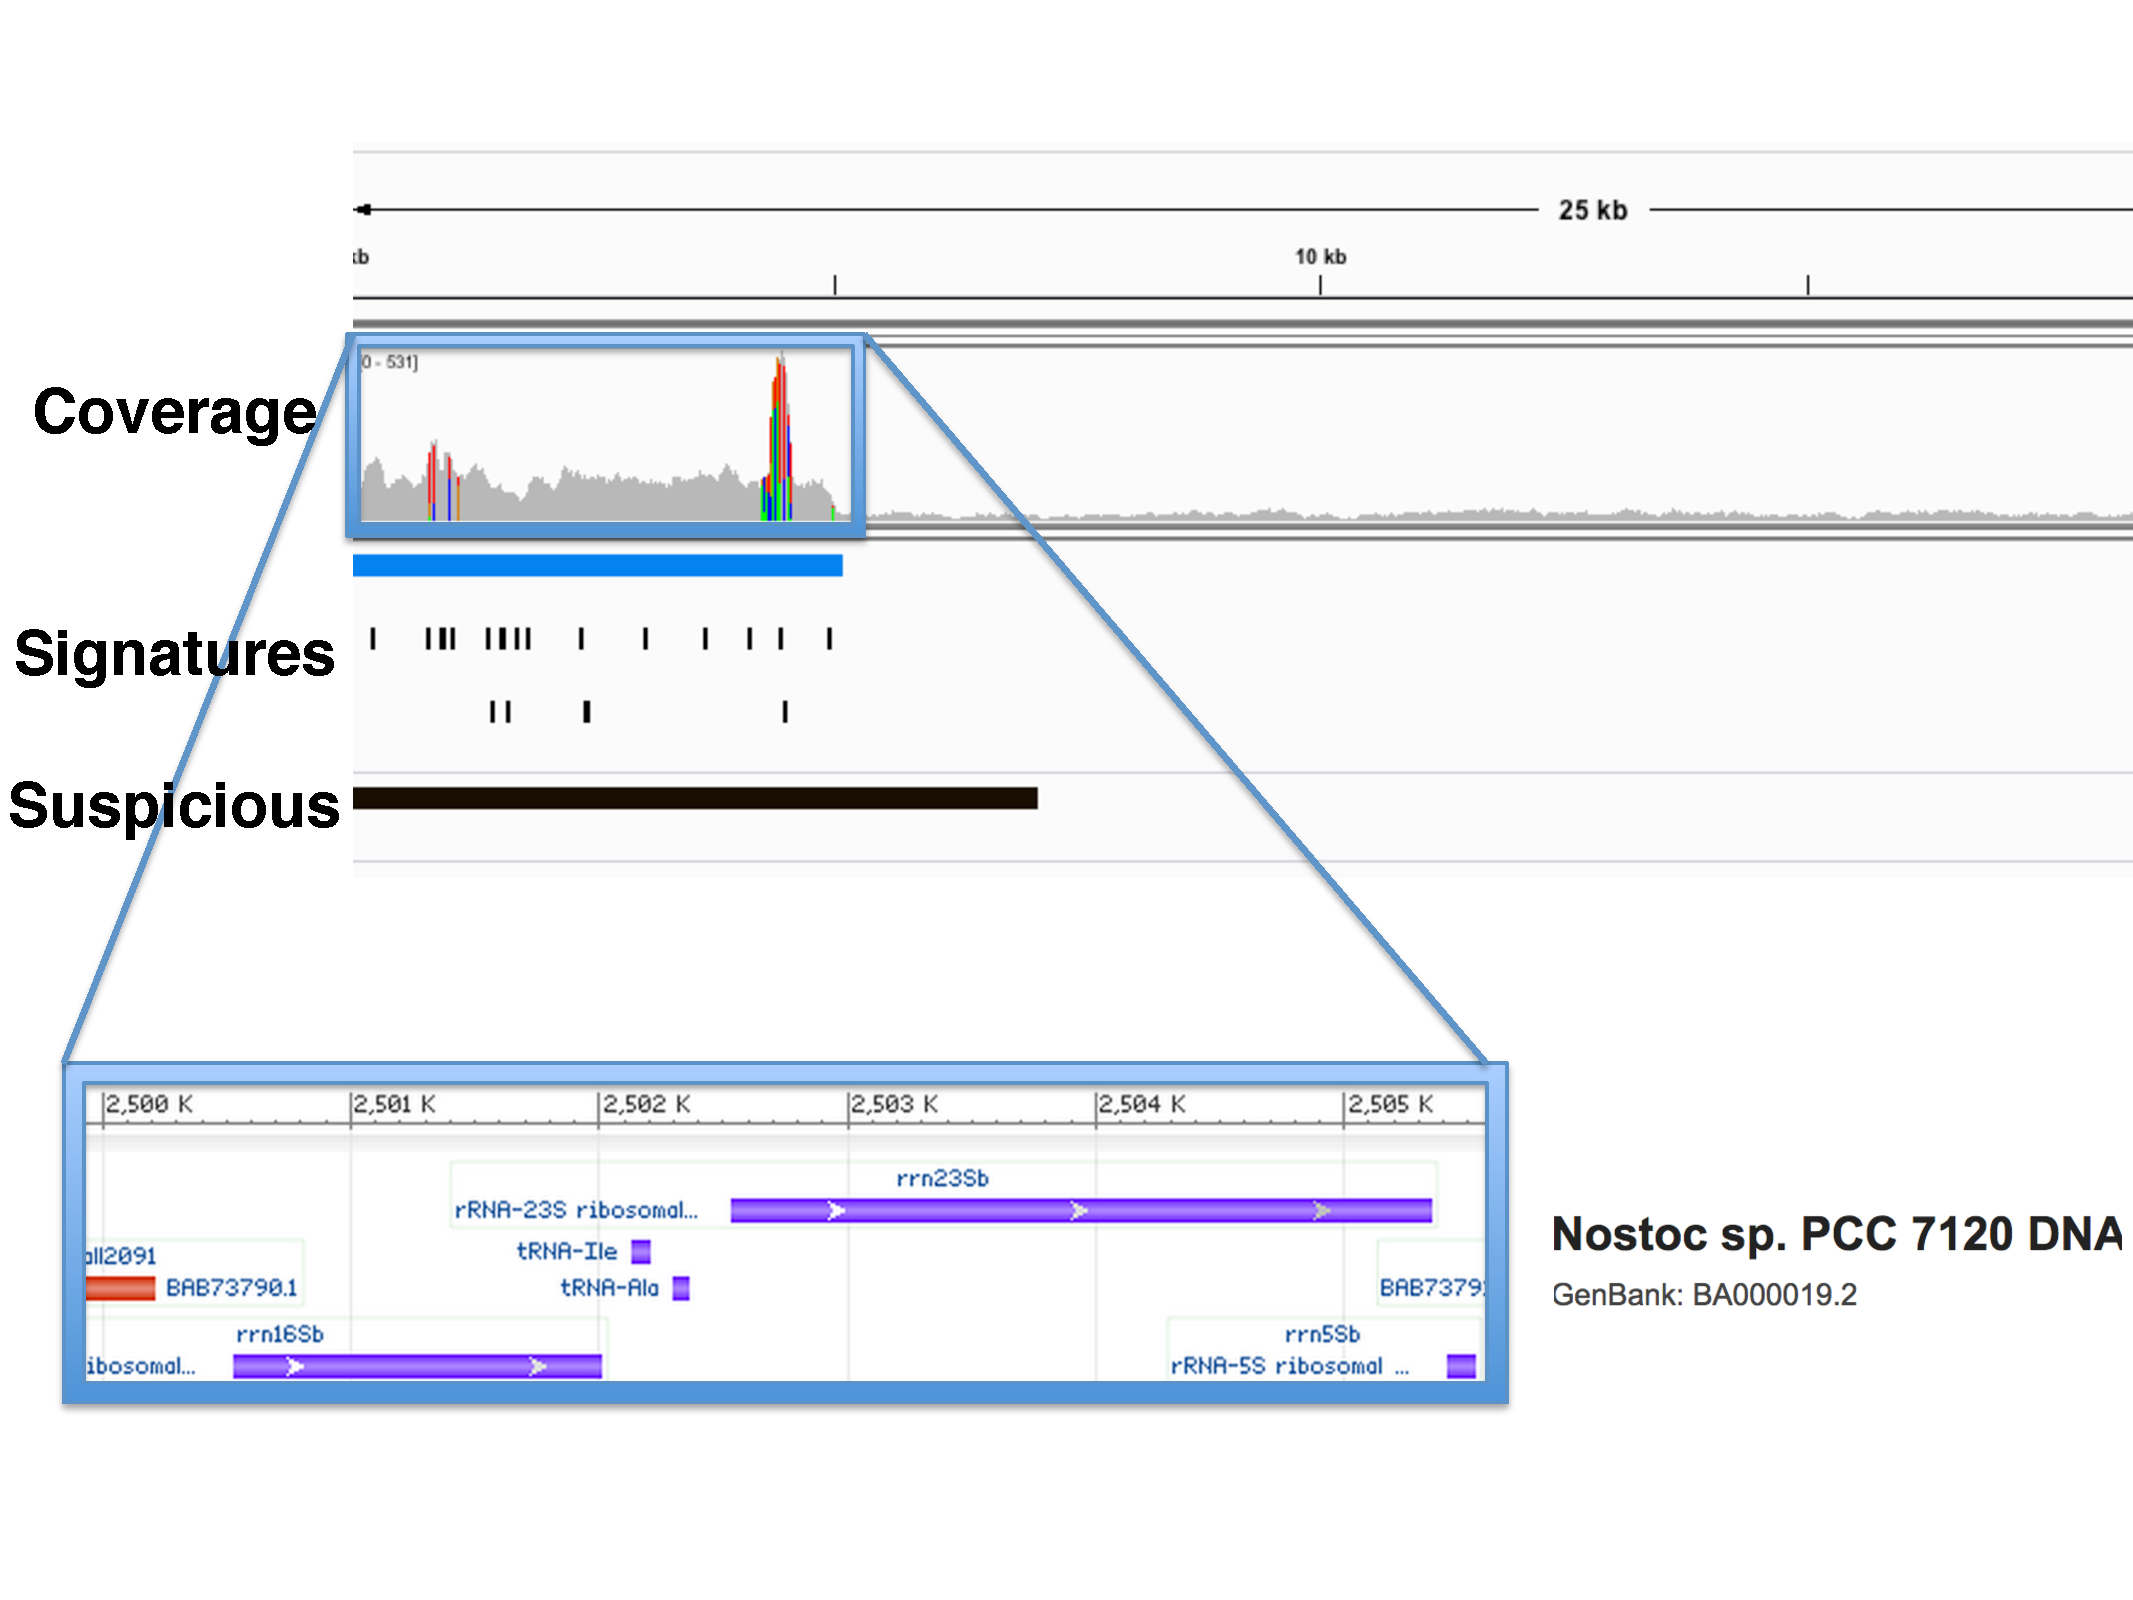
\includegraphics[width=4.86in]{figures/rrna_coverages}
\end{center}
\caption[Ribosomal genes found in region marked by VALET]{A closer examination of a region flagged by VALET, but no mis-assembly reported by QUAST. This region contained 16S, 23S, and 5S rRNA genes and was found at \emph{four} locations in the \emph{Nostoc} sp. PCC 7120 genome.}
\label{fig:rrna_misassembly}
\end{figure*}

Assemblathon1~\citep{earl2011assemblathon} has stated that assemblers have trouble with polymorphism and heterozygosity.
This problem is compounded in metagenomic assemblies due to closely-related strains having uneven abundances.
MetaCompass~\citep{metacompass}, a reference-based metagenomic assembler, was used to assemble the HMP Sample SRS024655 (retroauricular crease of a male).
A ~25 Kbp region was flagged as having low coverage by VALET, but not reported by QUAST (Figure~\ref{fig:p_acnes}).
After further investigation, the ~25 Kbp region belonged exclusively to the one of the reference genomes chosen by MetaCompass: \emph{Propionibacterium acnes} KPA171202.
The higher coverage flanking regions aligned to both \emph{Propionibacterium acnes} KPA171202 and \emph{Propionibacterium acnes} ATCC 11828.
\emph{Propionibacterium acnes} KPA171202 contains nearly 70 Kbp of insertions.
Despite being found at a lower abundance, the KPA171202 strain of \emph{Propionibacterium acnes} was chosen for the reference-guided assembly because all reads that were align to the ATCC 11828 strain also aligned to the KPA171202 strain.
Since the KPA171202 strain was actually found in the dataset, QUAST detected no structural errors.
A more \emph{correct} assembly would include both complete genomes.


\section{Conclusion}

VALET is the first \emph{de novo} pipeline for detecting mis-assemblies in metagenomic datasets.
VALET searches for regions of the assembly that are statistically inconsistent with characteristics of the data generation process.
VALET finds mis-assemblies on a simulated and synthetic metagenomic mock community.

\begin{figure*}[tb!]
\begin{center}
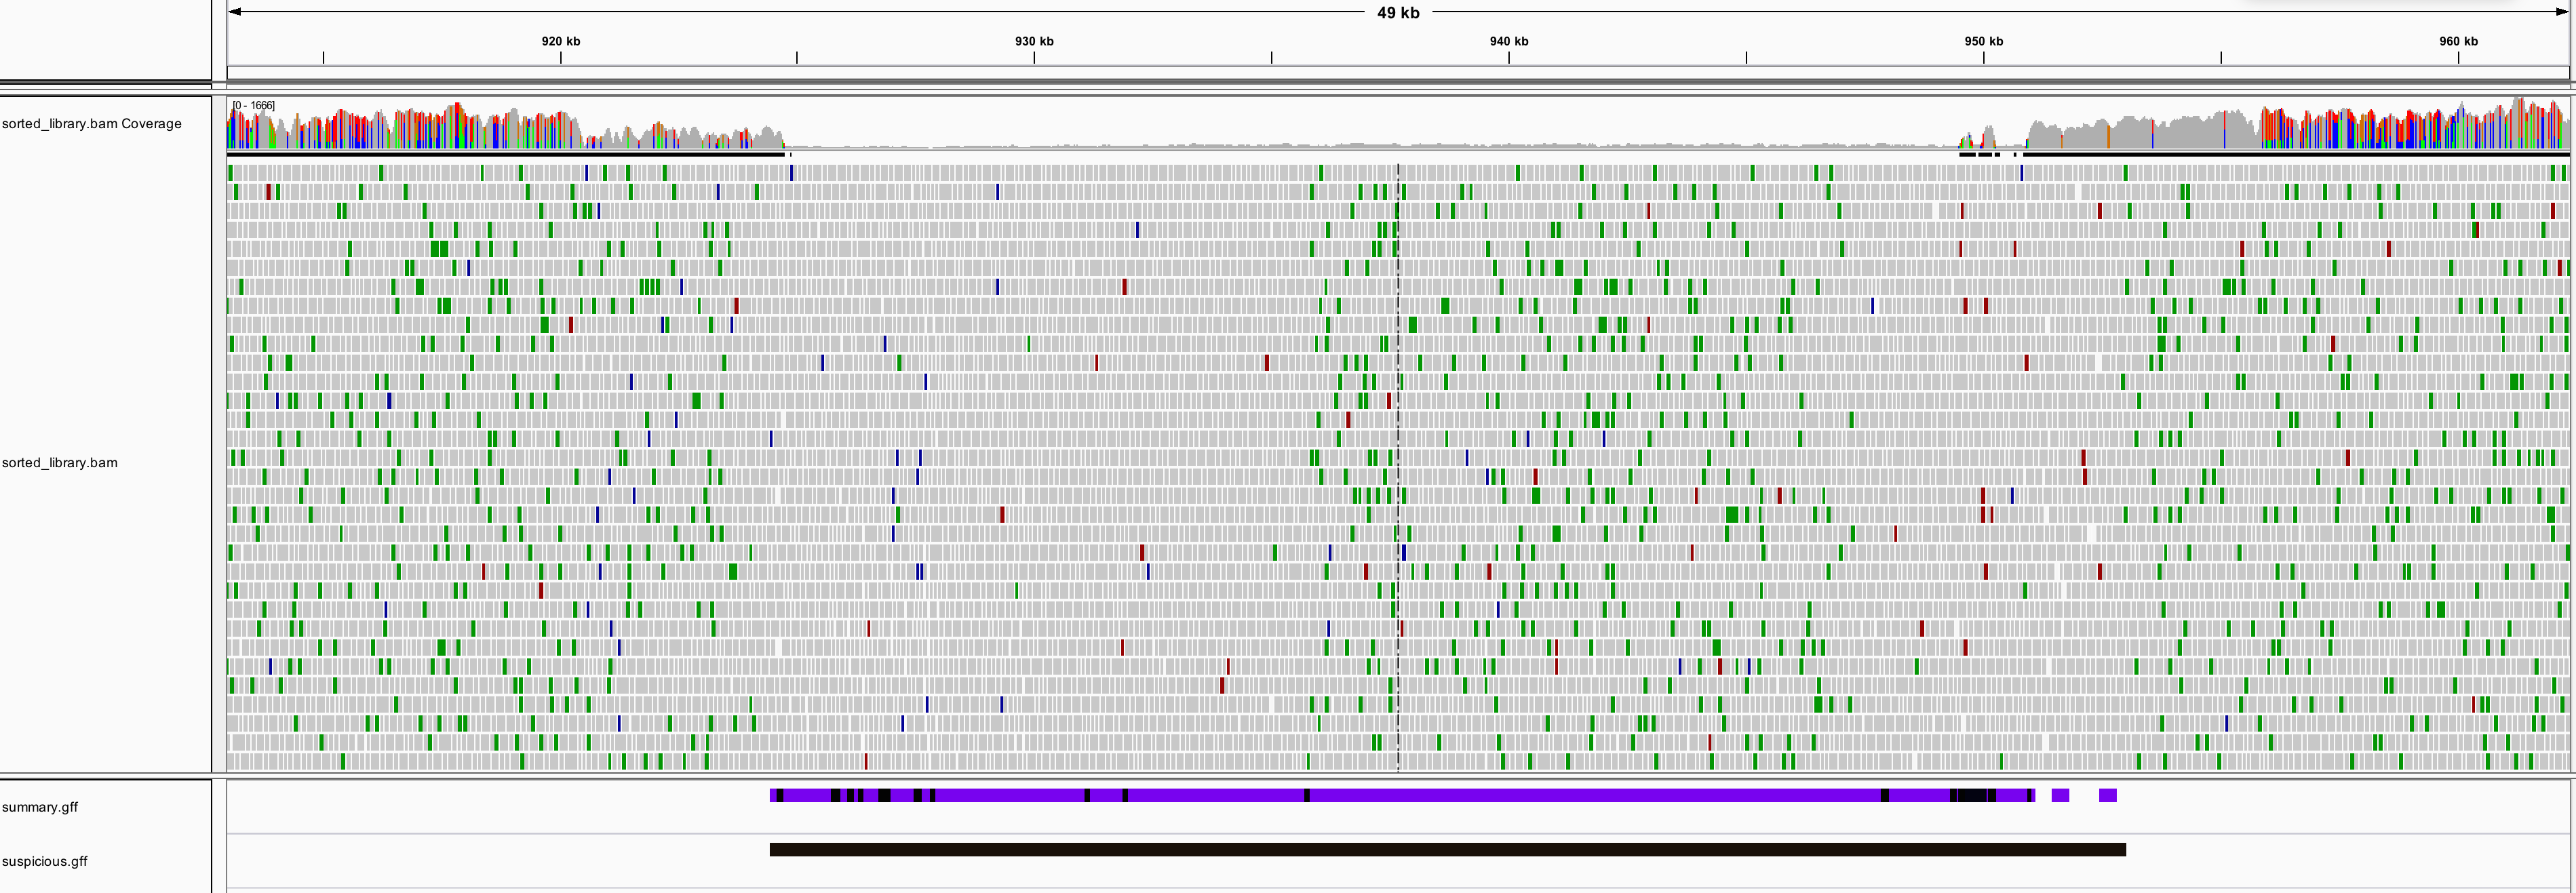
\includegraphics[width=1.4\textheight]{figures/p_acne_1}
\end{center}
\caption[Examining a 25 Kbp region flagged by VALET]{A 25 Kbp low coverage region flagged by VALET, but no mis-assembly reported by QUAST. The low coverage region was due to MetaCompass selecting only a single strain of \emph{Propionibacterium acnes} to use for assembly instead of both.}
\label{fig:p_acnes}
\end{figure*}

\section*{Acknowledgement}
=
\paragraph{Funding\textcolon} Text Text Text Text Text Text  Text Text.

\bibliographystyle{natbib}
\bibliographystyle{achemnat}
\bibliographystyle{plainnat}
\bibliographystyle{abbrv}
\bibliographystyle{bioinformatics}

\bibliographystyle{plain}

\bibliography{valet}

\end{document}
